\documentclass[11pt,letterpaper]{article}
\usepackage[lmargin=1in,rmargin=1in,bmargin=1in,tmargin=1in]{geometry}
\usepackage{style/quiz}
\usepackage{style/commands}

% -------------------
% Content
% -------------------
\begin{document}
\thispagestyle{title}


% Quiz 1
\quizsol \textit{True/False}: The following relation represents a function:
	\[
	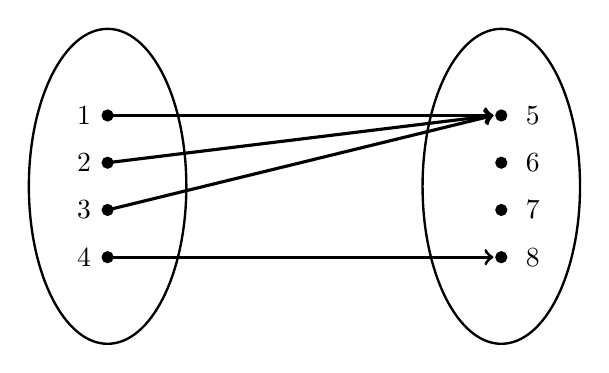
\begin{tikzpicture}
	% Ellipses
	\draw[line width=0.03cm] (0,0) circle (1 and 2);
	\draw[line width=0.03cm] (5,0) circle (1 and 2);
	
	% Nodes
	\draw[fill=black] (0,0.9) circle (0.07);
	\draw[fill=black] (0,0.3) circle (0.07);
	\draw[fill=black] (0,-0.3) circle (0.07);
	\draw[fill=black] (0,-0.9) circle (0.07);
	
	\draw[fill=black] (5,0.9) circle (0.07);
	\draw[fill=black] (5,0.3) circle (0.07);
	\draw[fill=black] (5,-0.3) circle (0.07);
	\draw[fill=black] (5,-0.9) circle (0.07);
	
	% Arrow
	\draw[line width=0.04cm,->] (0,0.9) -- (4.9,0.9);
	\draw[line width=0.04cm,->] (0,0.3) -- (4.9,0.9);
	\draw[line width=0.04cm,->] (0,-0.3) -- (4.9,0.9);
	\draw[line width=0.04cm,->] (0,-0.9) -- (4.9,-0.9);
	
	% Labels
	\node at (-0.3,0.9) {$1$};
	\node at (-0.3,0.3) {$2$};
	\node at (-0.3,-0.3) {$3$};
	\node at (-0.3,-0.9) {$4$};
	
	\node at (5.4,0.9) {$5$};
	\node at (5.4,0.3) {$6$};
	\node at (5.4,-0.3) {$7$};
	\node at (5.4,-0.9) {$8$};
	\end{tikzpicture}
	\]

\sol The statement is \textit{true}. A relation is a function if for every input, i.e. every value in the domain, there is one output. For each of the values 1, 2, 3, 4, we know the value of the output. It does not matter that several of the values get `sent' to the same value---only that we know what value they go to. \pvspace{1.5cm}



% Quiz 2
\quizsol \textit{True/False}: If $C(x)$ is a cost function, then the $y$-intercept of $C(x)$ is the fixed costs. \pspace

\sol The statement is \textit{true}. The $y$-intercept of a function is the value where $x= 0$ (which means the function is intersecting the $y$-axis). But then we are looking at the value of $C(0)$, which represents the costs of producing zero items. But any costs associated with producing zero items must be a `baseline' cost for production, i.e. the fixed costs. \pvspace{1.5cm}



% Quiz 3
\quizsol \textit{True/False}: The point $(1, 1)$ is the solution to the system of equations:
	\[
	\begin{aligned}
	2x + y&= 3 \\
	x - y&= 1
	\end{aligned}
	\]

\sol The statement is \textit{false}. The simplest way of seeing this is to check if $(x,y)= (1,1)$ is a solution to the system, i.e. check if $x= 1$ and $y= 1$ satisfies both equations: $2(1) + 1= 3$ but $1 - 1= 0 \neq 1$. Therefore, $(1, 1)$ is not the solution to the system of equations. We can also determine if $(1, 1)$ is a solution to the system of equations by solving the system: \par
	\begin{table}[!ht]
	\centering
	\begin{tabular}{cccc}
	& $2x + y$ & $=$ & $3$ \\
	& $x - y$ & $=$ & $1$ \\ \hline
	& $3x$ & $=$ & $4$ \\
	& $x$ & $=$ & $4/3$ 
	\end{tabular}
	\end{table}
Then certainly, we cannot have $x= 1$. We then can find that $y= x - 1= 4/3 - 1= 1/3$. Then the correct solution is $(x, y)= (4/3, 1/3)$. 



\newpage



% Quiz 4
\quizsol \text{True/False}: If $P(x)$ is a profit function, then $P(0)$ is a breakeven point. \pspace

\sol The statement is \textit{false}. Recall that a breakeven point is when revenue, $R(x)$, equals cost, $C(x)$. But this is $R(x)= C(x)$. This is the same as $R(x) - C(x)= 0$. But $P(x)= R(x) - C(x)$ so that $P(x)= 0$. Alternatively, a breakeven point can be defined as a $x$ value when the profit is 0, i.e. $P(x)= 0$. \pvspace{1.5cm}



















\end{document}